%%%%%%%%%%%%%%%%%%%%%%%%%%%%%%%%%%%%%%%
% Wenneker Resume/CV
% LaTeX Template
% Version 1.1 (19/6/2016)
%
% This template has been downloaded from:
% http://www.LaTeXTemplates.com
%
% Original author:
% Frits Wenneker (http://www.howtotex.com) with extensive modifications by 
% Vel (vel@LaTeXTemplates.com)
%
% License:
% CC BY-NC-SA 3.0 (http://creativecommons.org/licenses/by-nc-sa/3.0/
%
%%%%%%%%%%%%%%%%%%%%%%%%%%%%%%%%%%%%%%

%----------------------------------------------------------------------------------------
%	PACKAGES AND OTHER DOCUMENT CONFIGURATIONS
%----------------------------------------------------------------------------------------

\documentclass[a4paper,12pt]{memoir} % Font and paper size

\usepackage{contactinfo}
\usepackage{hyperref}
\hypersetup{
    colorlinks=true,
    linkcolor=blue,
    filecolor=magenta,
    urlcolor=cyan
    }

%%%%%%%%%%%%%%%%%%%%%%%%%%%%%%%%%%%%%%%%%
% Wenneker Resume/CV
% Structure Specification File
% Version 1.1 (19/6/2016)
%
% This file has been downloaded from:
% http://www.LaTeXTemplates.com
%
% Original author:
% Frits Wenneker (http://www.howtotex.com) with extensive modifications by 
% Vel (vel@latextemplates.com)
%
% License:
% CC BY-NC-SA 3.0 (http://creativecommons.org/licenses/by-nc-sa/3.0/)
%
%%%%%%%%%%%%%%%%%%%%%%%%%%%%%%%%%%%%%%%%%

%----------------------------------------------------------------------------------------
%	PACKAGES AND OTHER DOCUMENT CONFIGURATIONS
%----------------------------------------------------------------------------------------

\usepackage{XCharter} % Use the Bitstream Charter font
\usepackage[utf8]{inputenc} % Required for inputting international characters
\usepackage[T1]{fontenc} % Output font encoding for international characters

\usepackage[top=1cm,left=1cm,right=1cm,bottom=1cm]{geometry} % Modify margins

\usepackage{graphicx} % Required for figures

\usepackage{flowfram} % Required for the multi-column layout

\usepackage{url} % URLs

\usepackage[usenames,dvipsnames]{xcolor} % Required for custom colours

\usepackage{tikz} % Required for the horizontal rule

\usepackage{enumitem} % Required for modifying lists
\setlist{noitemsep,nolistsep} % Remove spacing within and around lists

\setlength{\columnsep}{\baselineskip} % Set the spacing between columns

% Define the left frame (sidebar)
\newflowframe{0.2\textwidth}{\textheight}{0pt}{0pt}[left]
\newlength{\LeftMainSep}
\setlength{\LeftMainSep}{0.2\textwidth}
\addtolength{\LeftMainSep}{1\columnsep}
 
% Small static frame for the vertical line
\newstaticframe{1.5pt}{\textheight}{\LeftMainSep}{0pt}
 
% Content of the static frame with the vertical line
\begin{staticcontents}{1}
\hfill
\tikz{\draw[loosely dotted,color=RoyalBlue,line width=1.5pt,yshift=0](0,0) -- (0,\textheight);}
\hfill\mbox{}
\end{staticcontents}
 
% Define the right frame (main body)
\addtolength{\LeftMainSep}{1.5pt}
\addtolength{\LeftMainSep}{1\columnsep}
\newflowframe{0.7\textwidth}{\textheight}{\LeftMainSep}{0pt}[main01]

\pagestyle{empty} % Disable all page numbering

\setlength{\parindent}{0pt} % Stop paragraph indentation

%----------------------------------------------------------------------------------------
%	NEW COMMANDS
%----------------------------------------------------------------------------------------

\newcommand{\userinformation}[1]{\renewcommand{\userinformation}{#1}} % Define a new command for the CV user's information that goes into the left column

\newcommand{\cvheading}[1]{{\Huge\bfseries\color{RoyalBlue} #1} \par\vspace{.6\baselineskip}} % New command for the CV heading
\newcommand{\cvsubheading}[1]{{\Large\bfseries #1} \bigbreak} % New command for the CV subheading

\newcommand{\Sep}{\vspace{1em}} % New command for the spacing between headings
\newcommand{\SmallSep}{\vspace{0.5em}} % New command for the spacing within headings

\newcommand{\aboutme}[2]{ % New command for the about me section
\textbf{\color{RoyalBlue} #1}~~#2\par\Sep
}
	
\newcommand{\CVSection}[1]{ % New command for the headings within sections
{\Large\textbf{#1}}\par
\SmallSep % Used for spacing
}

\newcommand{\CVItem}[2]{ % New command for the item descriptions
\textbf{\color{RoyalBlue} #1}\par
#2
\SmallSep % Used for spacing
}

\newcommand{\bluebullet}{\textcolor{RoyalBlue}{$\circ$}~~} % New command for the blue bullets
 % Include the file specifying document layout and packages


%----------------------------------------------------------------------------------------
%	NAME AND CONTACT INFORMATION 
%----------------------------------------------------------------------------------------

\newcommand{\fakecontact}{
(000) 111-1111 \\ % Your phone number
\Sep % Some whitespace
\textbf{Address} \\
123 Broadway \\ % Address 1
City, State 12345 \\ % Address 2
Country \\ % Address 3
}

\userinformation{ % Set the content that goes into the sidebar of each page
\begin{flushright}
% Comment out this figure block if you don't want a photo
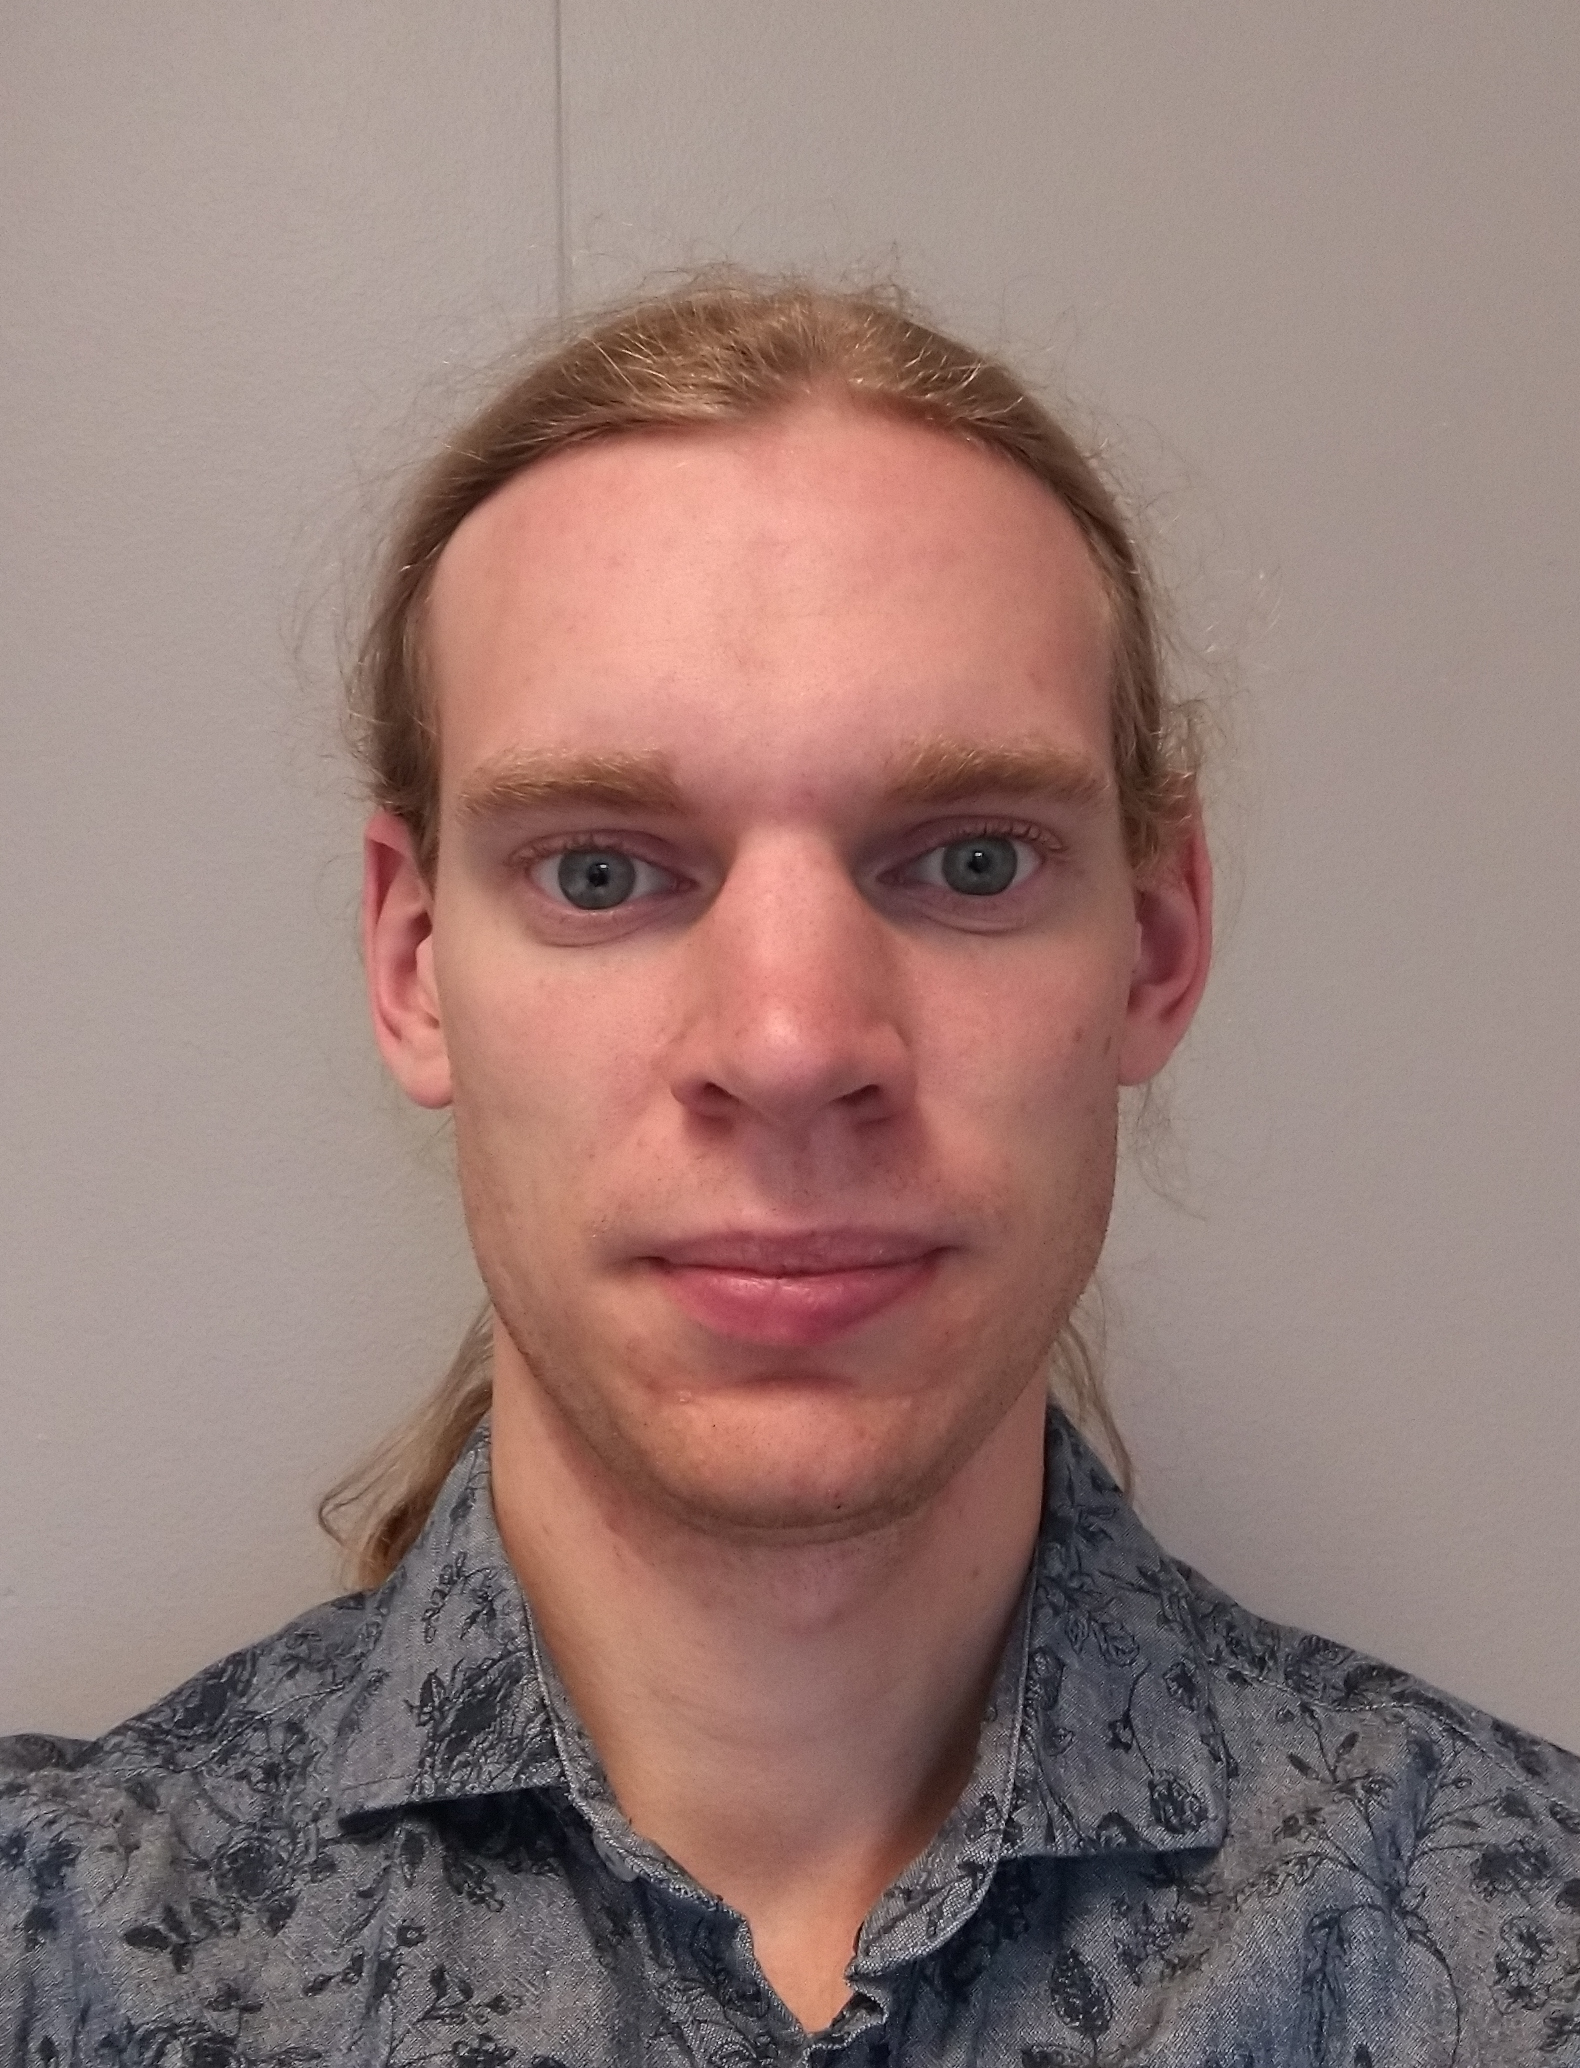
\includegraphics[width=0.6\columnwidth]{photo.jpg}\\[\baselineskip] % Your photo
\small % Smaller font size
Herman Lundkvist \\ % Your name
Born September, 1993 \\
\textbf{Contact} \\
\url{herman.lundkvist@gmail.com} \\ % Your email address
%\fakecontact
\realcontact
\Sep % Some whitespace
\textbf{Spoken Languages} \\
    Swedish \\
    English
\vfill % Whitespace under this block to push it up under the photo
\end{flushright}
}

%----------------------------------------------------------------------------------------

\begin{document}

\userinformation % Print your information in the left column

\framebreak % End of the first column

%----------------------------------------------------------------------------------------
%	HEADING
%----------------------------------------------------------------------------------------

\cvheading{Herman Lundkvist} % Large heading - your name

\cvsubheading{Software Engineer} % Subheading - your occupation/specialization

%----------------------------------------------------------------------------------------
%	ABOUT ME
%----------------------------------------------------------------------------------------

\aboutme{About Me}{
I thrive on problem-solving and deep diving into interesting subjects.
On my own I am resourceful and disciplined.
As a teammate I am diplomatic; I often try to listen others.
Professionally I am, among other things, 
interested in software close to the hardware.
On my spare time I enjoy mountain-biking in my local bike club.
Occassionaly I also work on some hobby programming and electronics projects,
such as a 3D-printed keyboard with a custom PCB I use as my daily driver.
}

%----------------------------------------------------------------------------------------
%	EDUCATION
%----------------------------------------------------------------------------------------

\CVSection{Education}

%------------------------------------------------
\CVItem{2014 - 2018, Linköping University}{MS in Computer Science and Engineering, thesis: \href{http://liu.diva-portal.org/smash/record.jsf?pid=diva2\%3A1191000&dswid=5587}{Accelerated Simulation of Modelica Models Using an FPGA-Based Approach}}

\CVItem{2015, Eindhoven University of Technology}{Studies abroad during the Autumn Semester}

\CVItem{2012 - 2014, Linköping University}{BS in Computer Science and Engineering}

%------------------------------------------------

\Sep % Extra whitespace after the end of a major section

%----------------------------------------------------------------------------------------
%	EXPERIENCE
%----------------------------------------------------------------------------------------

\CVSection{Full-Time Employment}

%------------------------------------------------

\CVItem{Dec 2019 - present, \textit{Software Developer}, Vector Sweden (VecScan AB)}{
\begin{itemize}
    \item implementation of Adaptive MICROSAR, a framework for developing software for high performance ECUs
    \item software development primarily in C++ and Java for Linux
    \item maintenance and implementon of \href{https://www.autosar.org/fileadmin/user\_upload/standards/adaptive/20-11/AUTOSAR\_SWS\_AdaptiveCore.pdf}{Adaptive Core}
    \item work on code generators used in Adaptive MICROSAR
\end{itemize}
}

\CVItem{Sep 2017 - dec 2019, \textit{Systems Engineer}, Saab AB}{
\begin{itemize}
    \item software development primarily in C and C++ for Unix and Unix-like platforms for the aircraft simulation department
	\item solo development of a Solaris driver for a CAN-bus PCIe-card
\end{itemize}
}

%------------------------------------------------
\CVSection{Internships}

\CVItem{Jun 2016 - Aug 2016, \textit{Summer Intern}, Saab AB}{
    Worked with development of an Ada-parser for the tool Doxygen.
}

\CVItem{Jun 2015 - Jul 2015, \textit{Summer Intern}, Ericsson AB}{
    Developed a python tool for automating analysis of logs from Ericsson base stations for the purpose of troubleshooting. 
}

\CVItem{Jun 2014 - Aug 2014, \textit{Summer Intern}, Sumline AB}{
    Worked at a start-up with development of a webscraper in python.
}

%------------------------------------------------

\Sep % Extra whitespace after the end of a major section

%----------------------------------------------------------------------------------------
%	SKILLS
%----------------------------------------------------------------------------------------

\CVSection{Software Development Skills}

%------------------------------------------------

\CVItem{Programming Languages of Most Proficiency}
{
\begin{tabular}{p{0.2\textwidth} p{0.2\textwidth} p{0.2\textwidth}}
    \bluebullet C &  \bluebullet C++ & \bluebullet Bash \\
    \bluebullet Java &  \bluebullet Python & \bluebullet Make\\
\end{tabular}
}

%------------------------------------------------

\CVItem{Development and Target Platforms of Most Familiarty}
{
\begin{tabular}{p{0.30\textwidth} p{0.3\textwidth} p{0.2\textwidth}}
    \bluebullet Linux (x86) & \bluebullet Solaris (x86 and SPARC)\\
\end{tabular}
}

%------------------------------------------------

\Sep % Extra whitespace after the end of a major section

%----------------------------------------------------------------------------------------
%	NEW PAGE DELIMITER
%	Place this block wherever you would like the content of your CV to go onto the next page
%----------------------------------------------------------------------------------------
%
%\clearpage % Start a new page
%
%\userinformation % Print your information in the left column
%
%\framebreak % End of the first column
%
\end{document}
